\documentclass[varwidth, border=5pt]{standalone}

% Diamond Model of Intrusion Analysis
%   - https://apps.dtic.mil/sti/pdfs/ADA586960.pdf
%   - https://www.recordedfuture.com/blog/diamond-model-intrusion-analysis
%   - FOR578 (2025), Book 2, Page 28

\usepackage[utf8]{inputenc}
\usepackage[T1]{fontenc}
\usepackage{tikz}
\usetikzlibrary{positioning}

\tikzset{edge label/.style={midway, sloped, font=\itshape\small, text=gray}}

\begin{document}

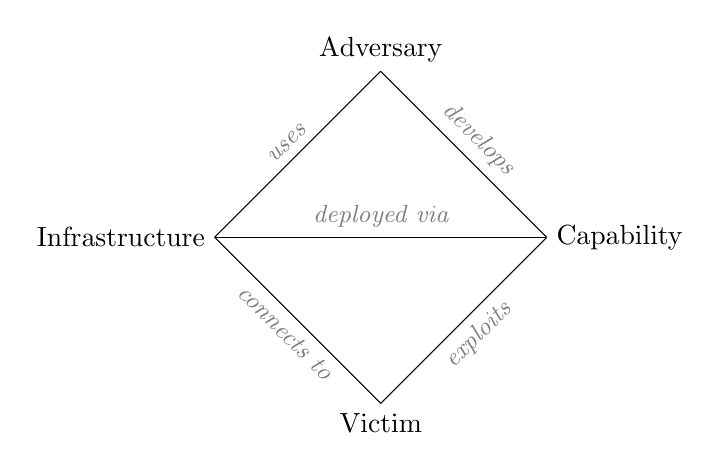
\begin{tikzpicture}[node distance=6em]

\coordinate (core) at (0, 0);

% Vertex labels
\node[above=of core, anchor=south] (adversary) {Adversary};
\node[right=of core, anchor=west] (capability) {Capability};  % or TTP
\node[below=of core, anchor=north] (victim) {Victim};
\node[left=of core, anchor=east] (infrastructure) {Infrastructure};

% Draw diamond with edge labels
\draw (infrastructure.east) -- node[edge label, above] {uses} (adversary.south);
\draw (adversary.south) -- node[edge label, above] {develops} (capability.west);
\draw (infrastructure.east) -- node[edge label, above] {deployed via} (capability.west);
\draw (infrastructure.east) -- node[edge label, below] {connects to} (victim.north);
\draw (victim.north) -- node[edge label, below] {exploits} (capability.west);

\end{tikzpicture}

\end{document}